\documentclass[conference]{IEEEtran}
\IfFileExists{cite.sty}{\usepackage{cite}}{}
\usepackage[T1]{fontenc}
\usepackage[utf8]{inputenc}
\usepackage{amsmath,amssymb}
\usepackage{graphicx}
\usepackage{booktabs}
\usepackage{array}
\usepackage{xcolor}
\usepackage{url}
\renewcommand{\ttdefault}{lmtt} % Courier no viene en TinyTeX; Latin Modern Mono si

\graphicspath{{figures/}}

% Marca visible de lo que todavia depende de los experimentos (T22-T25). Se quita en T28.
\newcommand{\pending}[1]{\textcolor{gray}{\textit{[Pending: #1]}}}

\begin{document}

\title{Machine Learning versus the Hedonic Model for House Price Prediction: A Reproducible Comparison on the Windsor Housing Data}

\author{\IEEEauthorblockN{Juan Miguel Le\'on G\'omez, Mauricio Jos\'e Mozo Ter\'an, and Brandon Eduardo Tobar S\'anchez}
\IEEEauthorblockA{Master's Program in Data Science and Artificial Intelligence\\
Universidad Aut\'onoma de Occidente, Cali, Colombia}}

\maketitle

% ---------------------------------------------------------------------------
\begin{abstract}
House prices drive mortgage lending, property taxation and household wealth, and they are still commonly estimated with linear hedonic regression. This paper compares the hedonic model with regularized, instance-based, kernel and tree-ensemble regressors on a classical benchmark: 545 house sales from Windsor, Canada, described by twelve structural and location attributes. We first verify the provenance of the public version of the data against the original econometric source, and then evaluate three preprocessing strategies and six models under repeated nested cross-validation, with a sealed test partition used only once. Models are compared on prediction error, computational cost and interpretability, where SHAP values are used to measure the impact of each attribute on the predictions. \pending{main quantitative results and conclusion, T22--T25.} All code, data and results are publicly available.
\end{abstract}

\begin{IEEEkeywords}
house price prediction, hedonic regression, automated valuation models, gradient boosting, random forest, explainability
\end{IEEEkeywords}

% ---------------------------------------------------------------------------
\section{Introduction}

The price of a house summarizes the value that the market assigns to a bundle of attributes: lot size, number of rooms, amenities and location. Hedonic price theory formalizes this idea by treating the price of a differentiated good as a function of its characteristics, each with an implicit price~\cite{rosen1974}. For decades this function has been estimated with linear or log-linear regression.

Estimating that price accurately has direct economic consequences. Housing is the main asset of most households: owner-occupied housing represents about half of household gross wealth on average across OECD countries, and more than 60\% for middle-class households~\cite{oecd2022}. The estimated value of a property determines the size of a mortgage loan, the base of the property tax and the reference price for buyers and sellers. Manual appraisal is slow, costly and dependent on the appraiser, which is why automated valuation models (AVMs) are standardized for mass appraisal~\cite{iaao2018} and can reach absolute errors close to 9\%, comparable to traditional appraisals~\cite{kok2017}. The need is especially visible in Colombia, where a 2019 national diagnosis found that only 5.68\% of the territory had up-to-date cadastral information~\cite{conpes3958}. Updating valuations at that scale requires methods that are reliable, reproducible and auditable.

The linear hedonic model is interpretable but imposes a rigid functional form with additive effects and no interactions. Machine learning (ML) models capture nonlinearities and interactions, but they can overfit small samples, are more expensive to train and are less transparent. The practical problem is therefore to decide, with evidence, which approach offers the best balance between prediction error, computational cost and interpretability.

This paper addresses the following question: \emph{to what extent do machine learning models improve the prediction of house sale prices over the linear hedonic model, using only structural and location attributes, and which attributes have the largest impact on their predictions?} The second part of the question is about the model, not about the market: we measure how much each attribute contributes to a prediction, and we make no causal claim about how prices are formed.

We study this question on the Windsor housing data of Anglin and Gen\c{c}ay~\cite{anglin1996}, a classical benchmark of hedonic econometrics. Its public version is widely used in tutorials, usually without reference to its origin. Three hypotheses guide the experiments:
\begin{itemize}
  \item \textbf{H1}: at least one tree ensemble achieves a lower cross-validated RMSE than the linear hedonic model.
  \item \textbf{H2}: modeling the logarithm of the price reduces the relative error (MAPE) of linear and distance-based models.
  \item \textbf{H3}: the attribute \texttt{furnishingstatus}, which is absent from the original data, does not significantly reduce the RMSE once the eleven original attributes are included.
\end{itemize}

The contributions of this work are: (i) a verified account of the provenance of the public dataset, including its exact relation to the original source; (ii) a factorial comparison of three preprocessing strategies and six regression models under the same cross-validation folds, with statistical tests; (iii) an analysis of computational complexity and of attribute impact with SHAP; and (iv) a fully reproducible repository~\cite{repo}.

The rest of the paper is organized as follows. Section~\ref{sec:related} reviews related work. Section~\ref{sec:data} describes the dataset and how it was obtained. Section~\ref{sec:problem} states the learning problem. Sections~\ref{sec:method} to~\ref{sec:conclusions} present the methodology, the results, the discussion and the conclusions.

% ---------------------------------------------------------------------------
\section{Related Work}
\label{sec:related}

We searched the literature following the PRISMA 2020 guideline~\cite{page2021}. Twenty queries over eleven academic sources returned 182 records, plus 10 identified through citations. After removing 66 duplicates and screening 116 records, 26 studies were included. Eligibility was assessed mainly on abstracts and metadata; three studies were read in full. The protocol, the search log and the complete literature matrix are available in the repository~\cite{repo}. Table~\ref{tab:literature} summarizes representative studies.

\begin{table}[t]
\caption{Representative Studies on House Price Prediction}
\label{tab:literature}
\centering
\footnotesize
\begin{tabular}{@{}>{\raggedright\arraybackslash}p{1.95cm}>{\raggedright\arraybackslash}p{2.1cm}>{\raggedright\arraybackslash}p{3.6cm}@{}}
\toprule
Study & Data & Main finding \\
\midrule
Anglin and Gen\c{c}ay~\cite{anglin1996} & Windsor, Canada; 546 sales & Semiparametric model predicts better than the parametric benchmark \\
Haupt \emph{et al.}~\cite{haupt2010} & Same Windsor data & A well-chosen parametric specification need not be rejected \\
Antipov and Pokryshevskaya~\cite{antipov2012} & Apartments, Russia & Random forest outperforms the compared methods \\
\v{C}eh \emph{et al.}~\cite{ceh2018} & Ljubljana; 7,407 sales & Random forest beats multiple regression \\
Valier~\cite{valier2020} & Review of comparisons & ML more accurate in 57 comparisons, regression in 13 \\
Ho \emph{et al.}~\cite{ho2021} & Hong Kong; $\approx$40,000 sales & Random forest and boosting outperform SVM \\
Stang \emph{et al.}~\cite{stang2022} & Germany; 1.2 million homes & XGBoost most accurate; OLS and GAM remain close \\
Kim and Hong~\cite{kim2024} & Jeju, Korea; 63,306 sales & Stacked ensemble beats single models \\
P\'erez-Rave \emph{et al.}~\cite{perezrave2020} & Colombia; 15,177 apartments & Ensembles have higher predictive power \\
Grinsztajn \emph{et al.}~\cite{grinsztajn2022} & 45 tabular datasets & Tree-based models outperform deep learning \\
\bottomrule
\end{tabular}
\end{table}

\subsection{Hedonic and Machine Learning Models}

Most of the reviewed studies report an advantage of tree ensembles over regression. Random forest outperforms multiple regression in Ljubljana~\cite{ceh2018} and the competing methods in a Russian apartment market~\cite{antipov2012}; random forest and bagging outperform simpler models in Colombia~\cite{perezrave2020}; XGBoost is the most accurate model in a nationwide German study~\cite{stang2022}; and a stacked ensemble beats individual algorithms in Korea~\cite{kim2024}. A review of published comparisons counts 57 cases favorable to ML against 13 favorable to regression~\cite{valier2020}.

The advantage is not uniform. In~\cite{stang2022}, a generalized additive model ($R^2 = 0.8664$) and OLS ($R^2 = 0.8654$) stay close to XGBoost ($R^2 = 0.8995$). In three intermediate Colombian cities, random forest achieves the lowest MAPE with ridge regression very close behind~\cite{rossomateus2022}. Most relevant for this paper, the econometric literature on the Windsor data compares parametric, semiparametric and nonparametric specifications~\cite{anglin1996,parmeter2007,haupt2010} and concludes that a well-chosen parametric model need not be rejected~\cite{haupt2010}. The hedonic model is therefore a strong baseline on this dataset, not a straw man. Finally, on tabular data of medium size, tree-based models remain ahead of deep neural networks~\cite{grinsztajn2022}, which supports leaving deep learning out of a study with 545 observations.

\subsection{Preprocessing, Validation and Metrics}

Preprocessing is reported unevenly. The studies we could verify describe outlier cleaning and georeferencing~\cite{stang2022}, feature selection~\cite{yalpir2021}, attributes derived from text~\cite{perezrave2020}, and imputation and scaling of web-scraped listings~\cite{rossomateus2022}. In the texts we accessed we found no systematic comparison of several preprocessing strategies over the same data and models.

Validation schemes and metrics also vary: RMSE, MSE and MAPE in~\cite{ho2021}; MAPE and $R^2$ among others in~\cite{stang2022}; accuracy in a study that casts the task as classification~\cite{park2015}. Steurer \emph{et al.}~\cite{steurer2021} classify 48 metrics into seven groups and warn that the chosen metric can change the winning model, and Mullainathan and Spiess~\cite{mullainathan2017} stress that ML should be judged on out-of-sample prediction. We therefore report several metrics and use repeated cross-validation with statistical tests.

\subsection{Interpretability}

Interpretability appears as the counterweight of ML: ML predicts better, while econometric models offer better inference~\cite{valier2020}. The techniques found in the review include sensitivity analysis~\cite{dimopoulos2019}, segment diagnostics with CART~\cite{antipov2012} and explainable AI applied to an ensemble~\cite{deng2025}.

\subsection{Gap}

On the Windsor benchmark, the published comparisons are econometric~\cite{anglin1996,parmeter2007,haupt2010}; in what we read, tree ensembles are not evaluated on it. In addition, the smallest sample among the ML studies with a verified size has 5,359 observations~\cite{park2015}, ten times larger than ours. This paper compares the hedonic model, regularized models and tree ensembles on the same small benchmark, and documents preprocessing, validation, cost and attribute impact explicitly.

% ---------------------------------------------------------------------------
\section{Dataset}
\label{sec:data}

\subsection{Source and Provenance}

The working file is the \emph{Housing Prices Dataset} published on Kaggle under a CC0 public-domain license~\cite{kaggle_housing}: 545 rows and 13 columns, with no accompanying documentation about its origin. We traced it to the data of Anglin and Gen\c{c}ay~\cite{anglin1996}: 546 sales of residential houses in Windsor, Ontario, Canada, during July, August and September of 1987, distributed with the \texttt{AER} package for R~\cite{kleiber2008}.

We verified the correspondence by code, comparing both files as multisets of rows:
\begin{itemize}
  \item \textbf{Price scale.} In all 545 rows, the Kaggle price equals the original price in 1987 Canadian dollars (CAD) multiplied by exactly 70.
  \item \textbf{Row count.} The original file contains one fully duplicated record; the public version has 545 rows because that duplicate was dropped.
  \item \textbf{Renamed attributes.} Eight attributes were renamed, in some cases changing their apparent meaning. For instance, \texttt{area} is the size of the lot and not the built area, \texttt{mainroad} indicates a driveway, and \texttt{guestroom} indicates a recreation room.
  \item \textbf{Added attribute.} \texttt{furnishingstatus} does not exist in the original data. It was added in the public version without any description of how it was produced.
\end{itemize}

This verification matters for two reasons. It gives each attribute its documented meaning, and it identifies one attribute of unknown origin, which motivates hypothesis H3.

\subsection{Variables}

Table~\ref{tab:variables} lists the target and the twelve predictors with their original names. Five predictors are numeric, six are binary and one is categorical with three levels. Throughout the paper, prices are reported in 1987 CAD, that is, the Kaggle value divided by 70.

\begin{table}[t]
\caption{Variables of the Dataset}
\label{tab:variables}
\centering
\footnotesize
\setlength{\tabcolsep}{3pt}
\begin{tabular}{@{}llp{2.75cm}l@{}}
\toprule
Kaggle name & Original & Description & Range \\
\midrule
\texttt{price} & \texttt{price} & Sale price (CAD, 1987) & 25k--190k \\
\texttt{area} & \texttt{lotsize} & Lot size (sq.\ ft) & 1,650--16,200 \\
\texttt{bedrooms} & \texttt{bedrooms} & Number of bedrooms & 1--6 \\
\texttt{bathrooms} & \texttt{bathrooms} & Full bathrooms & 1--4 \\
\texttt{stories} & \texttt{stories} & Stories above ground & 1--4 \\
\texttt{parking} & \texttt{garage} & Garage places & 0--3 \\
\texttt{mainroad} & \texttt{driveway} & Has a driveway & yes/no \\
\texttt{guestroom} & \texttt{recreation} & Has a recreation room & yes/no \\
\texttt{basement} & \texttt{fullbase} & Full finished basement & yes/no \\
\texttt{hotwaterheating} & \texttt{gasheat} & Gas for water heating & yes/no \\
\texttt{airconditioning} & \texttt{aircon} & Central air conditioning & yes/no \\
\texttt{prefarea} & \texttt{prefer} & Preferred neighborhood & yes/no \\
\texttt{furnishingstatus} & --- & Furnishing (added in Kaggle) & 3 levels \\
\bottomrule
\end{tabular}
\end{table}

\subsection{Data Quality}

The file is complete: it has no missing values and no duplicated rows, and every value lies within its valid domain. Four findings condition the experimental design:
\begin{itemize}
  \item The file is sorted by descending price, so rows must be shuffled before any split.
  \item Fifteen sales are high-price outliers under the $1.5 \times \text{IQR}$ rule. They are real transactions and are kept.
  \item \texttt{hotwaterheating} is rare: only 4.6\% of the 545 houses have it.
  \item Six groups of houses share identical attributes but different prices (sixteen if \texttt{furnishingstatus} is ignored). This is direct evidence of irreducible noise: no model can predict those differences from the available attributes.
\end{itemize}

\subsection{Sealed Test Partition}

Before any analysis of the relation between attributes and price, the data were split into 436 training rows (80\%) and 109 test rows (20\%), stratified by price quintiles with a fixed seed. The test partition is sealed: it is not used to explore, tune or select anything, and it is evaluated only once, for the final model. Binary attributes were encoded as 0/1 with fixed rules. Every transformation that learns from the data, such as scaling, is fitted inside the cross-validation folds (Section~\ref{sec:method}).

\subsection{Exploratory Analysis}

The exploratory analysis uses the training partition only. In this partition the median price is 62,000 CAD and the mean is 68,199 CAD. Fig.~\ref{fig:price} shows that the price is right-skewed (skewness 1.20) and that its logarithm is nearly symmetric (0.13), which motivates modeling the log price as one of the preprocessing strategies. Lot size is also right-skewed (1.33).

\begin{figure}[t]
\centering
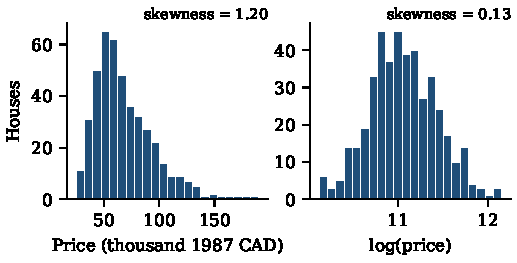
\includegraphics[width=\columnwidth]{fig_price_distribution.pdf}
\caption{Distribution of the sale price and of its logarithm in the training partition ($n = 436$).}
\label{fig:price}
\end{figure}

Fig.~\ref{fig:correlation} shows the Spearman correlation of each attribute with the price. Lot size (0.60), number of bathrooms (0.49) and central air conditioning (0.47) have the strongest association. No single attribute dominates, and \texttt{furnishingstatus} shows a moderate correlation (0.31) despite its undocumented origin.

\begin{figure}[t]
\centering
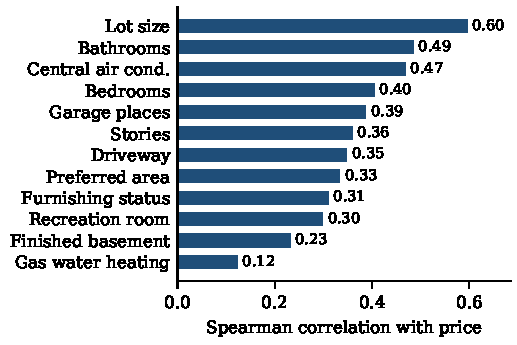
\includegraphics[width=\columnwidth]{fig_correlation_price.pdf}
\caption{Spearman correlation between each attribute and the sale price in the training partition.}
\label{fig:correlation}
\end{figure}

% ---------------------------------------------------------------------------
\section{Problem Formulation}
\label{sec:problem}

The task is \emph{supervised regression}. Each house $i$ is described by a vector $\mathbf{x}_i$ of twelve attributes and a continuous target $y_i > 0$, its sale price. Given the training set $\mathcal{D} = \{(\mathbf{x}_i, y_i)\}_{i=1}^{n}$ with $n = 436$, the goal is to learn a function $f$ that predicts the price of houses not seen during training:
\begin{equation}
  \hat{y} = f(\mathbf{x}), \qquad f^{*} = \arg\min_{f \in \mathcal{F}} \; \mathbb{E}\!\left[(y - f(\mathbf{x}))^{2}\right],
\end{equation}
where $\mathcal{F}$ is the family of functions of each model. The linear hedonic model restricts $\mathcal{F}$ to $f(\mathbf{x}) = \beta_0 + \boldsymbol{\beta}^{\top}\mathbf{x}$, or to its semi-logarithmic form when the target is $\log y$. The ML models enlarge $\mathcal{F}$ to nonlinear functions with interactions.

Models are trained by minimizing the squared error and evaluated, always on the original price scale, with the root mean squared error (RMSE), the mean absolute error (MAE), the mean absolute percentage error (MAPE) and the coefficient of determination ($R^2$):
\begin{equation}
  \text{RMSE} = \sqrt{\frac{1}{m}\sum_{i=1}^{m}(y_i - \hat{y}_i)^2}, \quad
  \text{MAPE} = \frac{100}{m}\sum_{i=1}^{m}\left|\frac{y_i - \hat{y}_i}{y_i}\right|.
\end{equation}

Because the sample is small, generalization is estimated with repeated cross-validation on the training partition, and the sealed test partition provides a single final estimate. The conclusions are predictive, not causal: an attribute with a large impact on the predictions is not necessarily a cause of the price.

% ---------------------------------------------------------------------------
% Las secciones siguientes se escriben en T28, cuando esten los resultados de T17-T25.
\section{Methodology}
\label{sec:method}
\pending{three preprocessing strategies (T17, T18), six models (T19--T21) and nested cross-validation with statistical tests (T22).}

\section{Experiments and Results}
\label{sec:results}
\pending{cross-validated comparison, ablation of \texttt{furnishingstatus}, and final evaluation on the sealed test partition (T22, T25).}

\section{Complexity Analysis}
\label{sec:complexity}
\pending{theoretical and empirical cost of each model (T23).}

\section{Discussion}
\label{sec:discussion}
\pending{error analysis and attribute impact with SHAP (T24); limitations: data from 1987 and one city, small sample, attribute of unknown origin.}

\section{Conclusions}
\label{sec:conclusions}
\pending{answers to H1--H3 and future work.}

\bibliographystyle{IEEEtran}
\bibliography{references}

\end{document}
